\documentclass[11pt,a4paper]{article}
\usepackage[utf8]{inputenc}
\usepackage[T1]{fontenc}
\usepackage{lmodern}
\usepackage[margin=2.5cm]{geometry}
\usepackage{amsmath,amssymb,amsthm}
\usepackage{graphicx}
\usepackage{hyperref}
\hypersetup{colorlinks=false,pdfborder={0 0 0}}

\newtheorem{theorem}{Theorem}
\newtheorem{lemma}{Lemma}
\newtheorem{corollary}{Corollary}
\newtheorem{proposition}{Proposition}
\theoremstyle{definition}
\newtheorem{definition}{Definition}
\theoremstyle{remark}
\newtheorem{remark}{Remark}

\newcommand{\R}{\mathbb{R}}
\newcommand{\norm}[1]{\left\lVert #1 \right\rVert}
\newcommand{\ip}[2]{\left\langle #1, #2 \right\rangle}

\title{Convergence Rates of First-Order Methods:\\ Proofs and Numerical Experiments}
\author{Arthur Conche\\ M2 MMAS, Universit\'e Paris Cit\'e}
\date{Working draft --- \today}

\begin{document}
\maketitle

\begin{abstract}
This report studies the convergence of first-order optimization methods (gradient descent, Nesterov's accelerated gradient and stochastic gradient descent) for smooth functions. For each method we prove the classical convergence rate under convexity, strong convexity or the Polyak--{\L}ojasiewicz condition, and we compare these theoretical bounds with numerical experiments. \emph{[Draft: to be completed.]}
\end{abstract}

\section{Introduction}
\emph{[To be written: motivation, question studied, contributions, outline.]}

\section{Setting and assumptions}
We consider the unconstrained problem
\[
\min_{x \in \R^d} f(x),
\]
where $f : \R^d \to \R$ is differentiable, and we denote by $f^\ast = \inf f$ and by $x^\ast$ a minimizer when one exists.

\begin{definition}[$L$-smoothness]
Let $L > 0$. A differentiable function $f : \R^d \to \R$ is \emph{$L$-smooth} if its gradient is $L$-Lipschitz:
\[
\norm{\nabla f(x) - \nabla f(y)} \le L \norm{x - y} \qquad \text{for all } x, y \in \R^d.
\]
\end{definition}

\emph{[To add: convexity, $\mu$-strong convexity, condition number $\kappa = L/\mu$, Polyak--{\L}ojasiewicz condition.]}

\section{Preliminary results}

\begin{lemma}[Descent lemma]\label{lem:descent}
Let $f : \R^d \to \R$ be differentiable and $L$-smooth. Then for all $x, y \in \R^d$,
\[
f(y) \le f(x) + \ip{\nabla f(x)}{y - x} + \frac{L}{2}\norm{y - x}^2 .
\]
\end{lemma}

\begin{proof}
Since $\nabla f$ is $L$-Lipschitz, it is continuous, hence $f$ is of class $C^1$. Fix $x, y \in \R^d$ and set $\varphi(t) = f(x + t(y - x))$ for $t \in [0,1]$. The function $\varphi$ is $C^1$ with $\varphi'(t) = \ip{\nabla f(x + t(y-x))}{y - x}$, so by the fundamental theorem of calculus,
\[
f(y) - f(x) = \varphi(1) - \varphi(0) = \int_0^1 \ip{\nabla f(x + t(y-x))}{y - x} \, dt .
\]
Since $\int_0^1 \ip{\nabla f(x)}{y - x}\, dt = \ip{\nabla f(x)}{y - x}$, we obtain
\[
f(y) - f(x) - \ip{\nabla f(x)}{y - x} = \int_0^1 \ip{\nabla f(x + t(y-x)) - \nabla f(x)}{y - x} \, dt .
\]
By the Cauchy--Schwarz inequality, then $L$-smoothness,
\begin{align*}
\int_0^1 \ip{\nabla f(x + t(y-x)) - \nabla f(x)}{y - x} \, dt
&\le \int_0^1 \norm{\nabla f(x + t(y-x)) - \nabla f(x)} \, \norm{y - x} \, dt \\
&\le \int_0^1 L \norm{t(y - x)} \, \norm{y - x} \, dt \\
&= L \norm{y - x}^2 \int_0^1 t \, dt \qquad (\text{since } t \ge 0)\\
&= \frac{L}{2} \norm{y - x}^2 ,
\end{align*}
which gives the result.
\end{proof}

\begin{remark}
Convexity is not used in the proof: the descent lemma holds for every $L$-smooth function. This is what allows the analysis of gradient descent for non-convex functions satisfying the Polyak--{\L}ojasiewicz condition (Section~\ref{sec:pl}).
\end{remark}

\begin{remark}
Since the Cauchy--Schwarz inequality bounds the absolute value of the integrand, the same argument gives the two-sided bound
\[
\left| f(y) - f(x) - \ip{\nabla f(x)}{y - x} \right| \le \frac{L}{2}\norm{y - x}^2 \qquad \text{for all } x, y \in \R^d.
\]
\end{remark}

\begin{corollary}[Sufficient decrease]\label{cor:sufficient}
Let $f : \R^d \to \R$ be differentiable and $L$-smooth. For every $x \in \R^d$, the gradient step $x^+ = x - \frac{1}{L}\nabla f(x)$ satisfies
\[
f(x^+) \le f(x) - \frac{1}{2L}\norm{\nabla f(x)}^2 .
\]
\end{corollary}

\begin{proof}
Applying Lemma~\ref{lem:descent} with $y = x^+$, so that $x^+ - x = -\frac{1}{L}\nabla f(x)$, we get
\begin{align*}
f(x^+) &\le f(x) + \ip{\nabla f(x)}{-\tfrac{1}{L}\nabla f(x)} + \frac{L}{2}\norm{-\tfrac{1}{L}\nabla f(x)}^2 \\
&= f(x) - \frac{1}{L}\norm{\nabla f(x)}^2 + \frac{L}{2L^2}\norm{\nabla f(x)}^2 \\
&= f(x) - \frac{1}{2L}\norm{\nabla f(x)}^2 .
\end{align*}
\end{proof}

\begin{remark}
In particular, each gradient step with step size $1/L$ decreases $f$, strictly as long as $\nabla f(x) \neq 0$. As for Lemma~\ref{lem:descent}, convexity is not needed. Iterating the inequality along the gradient descent sequence $x_{k+1} = x_k - \frac{1}{L}\nabla f(x_k)$ gives the starting point of all the convergence proofs of Section~4.
\end{remark}

\section{Gradient descent}
Throughout this section, $(x_k)_{k \ge 0}$ denotes the gradient descent sequence with step size $1/L$:
\[
x_{k+1} = x_k - \frac{1}{L}\nabla f(x_k), \qquad k \ge 0.
\]

\subsection{The quadratic case: how tight is the sufficient decrease?}\label{sec:quadratic}
Let $A \in \mathcal{S}_d(\R)$ be symmetric positive definite, with smallest eigenvalue $\mu > 0$ and largest eigenvalue $L$, and let
\[
f(x) = \frac12 x^\top A x, \qquad \nabla f(x) = Ax .
\]
Then $f$ is $L$-smooth and $\mu$-strongly convex, with $x^\ast = 0$ and $f^\ast = 0$. To measure how much of the guaranteed decrease of Corollary~\ref{cor:sufficient} is actually achieved, we define, whenever $\nabla f(x_k) \neq 0$,
\[
r_k = \frac{f(x_k) - f(x_{k+1})}{\frac{1}{2L}\norm{\nabla f(x_k)}^2} .
\]
Corollary~\ref{cor:sufficient} states exactly that $r_k \ge 1$.

\begin{proposition}\label{prop:rk}
For every $k \ge 0$ such that $x_k \neq 0$,
\[
r_k = 2 - \frac{\ip{g_k}{A g_k}}{L \norm{g_k}^2} \qquad \text{where } g_k = \nabla f(x_k) = A x_k,
\]
and consequently
\[
1 \le r_k \le 2 - \frac{\mu}{L} = 2 - \frac{1}{\kappa}.
\]
\end{proposition}

\begin{proof}
Since $A$ is invertible, $x_k \neq 0$ implies $g_k \neq 0$, so $r_k$ is well defined. Write $x = x_k$ and $g = g_k = Ax$, so that $x_{k+1} = x - \frac{1}{L} g$.

\emph{Exact expression.} By definition of $r_k$ and of $f$,
\[
r_k = \frac{2L}{\norm{g}^2}\Big(\tfrac12 x^\top A x - \tfrac12 (x - \tfrac1L g)^\top A (x - \tfrac1L g)\Big)
= \frac{L}{\norm{g}^2}\Big(\ip{x}{Ax} - \ip{x - \tfrac1L g}{Ax - \tfrac1L Ag}\Big).
\]
Expanding the second inner product and using $Ax = g$,
\[
\ip{x - \tfrac1L g}{g - \tfrac1L Ag} = \ip{x}{g} - \frac1L \ip{x}{Ag} - \frac1L \ip{g}{g} + \frac{1}{L^2}\ip{g}{Ag}.
\]
Since $A$ is symmetric, $\ip{x}{Ag} = \ip{Ax}{g} = \norm{g}^2$, and $\ip{x}{Ax} = \ip{x}{g}$. Therefore
\[
r_k = \frac{L}{\norm{g}^2}\Big(\frac{2}{L}\norm{g}^2 - \frac{1}{L^2}\ip{g}{Ag}\Big) = 2 - \frac{\ip{g}{Ag}}{L\norm{g}^2}.
\]

\emph{Bounds.} By the spectral theorem, $A$ is diagonalizable in an orthonormal basis $(e_1, \dots, e_d)$ of eigenvectors, with eigenvalues $\lambda_1, \dots, \lambda_d \in [\mu, L]$. Writing $g = \sum_{i=1}^d \ip{g}{e_i} e_i$, we get $Ag = \sum_{i=1}^d \lambda_i \ip{g}{e_i} e_i$, hence
\[
\ip{g}{Ag} = \sum_{i=1}^d \lambda_i \ip{g}{e_i}^2 .
\]
Since $\mu \le \lambda_i \le L$ and $\sum_{i=1}^d \ip{g}{e_i}^2 = \norm{g}^2$ (Parseval's identity in an orthonormal basis),
\[
\mu \norm{g}^2 \le \ip{g}{Ag} \le L \norm{g}^2, \qquad\text{i.e.}\qquad \frac{\ip{g}{Ag}}{L\norm{g}^2} \in \Big[\frac{\mu}{L}, 1\Big].
\]
Plugging this into the exact expression gives $1 \le r_k \le 2 - \frac{\mu}{L}$.
\end{proof}

\begin{remark}
The quantity $\ip{g}{Ag}/\norm{g}^2$ is the Rayleigh quotient of $A$ at $g$. The lower bound $r_k = 1$ is attained when $g_k$ is an eigenvector for $L$: the sufficient decrease inequality is then tight. The upper bound $2 - 1/\kappa$ is attained when $g_k$ is an eigenvector for $\mu$. Along gradient descent, the components of $x_k$ along the eigenvector $e_i$ are multiplied by $(1 - \lambda_i/L)$ at each step, so the slowest direction (eigenvalue $\mu$) dominates for large $k$, and one expects $r_k \to 2 - 1/\kappa$. This is what we observe numerically (Section~\ref{sec:experiments}).
\end{remark}

\subsection{Convex case}
\emph{[R1: $f(x_k) - f^\ast \le \dfrac{L\norm{x_0 - x^\ast}^2}{2k}$.]}
\subsection{Strongly convex case}
\emph{[R2: $\norm{x_k - x^\ast}^2 \le (1 - 1/\kappa)^k \norm{x_0 - x^\ast}^2$.]}
\subsection{Polyak--{\L}ojasiewicz condition}\label{sec:pl}
\emph{[R4: linear rate without convexity.]}

\section{Nesterov's accelerated gradient}
\emph{[R3: $O(1/k^2)$ via a Lyapunov function; $(1 - 1/\sqrt{\kappa})^k$ in the strongly convex case; lower bound; ODE interpretation.]}

\section{Stochastic gradient descent}
\emph{[R5: constant step size and noise floor; decreasing step size and $O(1/k)$ rate.]}

\section{Numerical experiments}\label{sec:experiments}

\subsection{Gradient descent on quadratics}\label{sec:exp-quadratic}

\paragraph{Setting.}
We consider the quadratic $f(x) = \frac12 x^\top A x$ of Section~\ref{sec:quadratic} in dimension $d = 100$, with $\mu = 1$ and $L = \kappa$ for $\kappa \in \{10, 100, 1000\}$. The matrix $A$ is built as $A = Q D Q^\top$, where $D$ is diagonal with entries $\mu$, $L$ and $d-2$ values drawn uniformly in $[\mu, L]$, and $Q$ is the orthogonal factor of the QR factorization of a $d \times d$ matrix with i.i.d.\ standard Gaussian entries. By construction, the smallest and largest eigenvalues of $A$ are exactly $\mu$ and $L$. The starting point $x_0$ is a standard Gaussian vector, and we run $5000$ iterations of gradient descent with step size $1/L$. Since $f^\star = 0$, the optimality gap is $f(x_k)$ itself. Iterations with $f(x_k) < 10^{-12}$ are discarded from the plots and the statistics below: at that level, the differences $f(x_k) - f(x_{k+1})$ are dominated by floating-point rounding errors. All random quantities are drawn from a single generator with a fixed seed, and the figures are produced by the script \texttt{code/experiments/exp01\_gd\_quadratic.py}. Before the experiment, the gradient $\nabla f(x) = Ax$ was checked against central finite differences (maximal relative error of order $10^{-10}$).

\begin{figure}[ht]
\centering
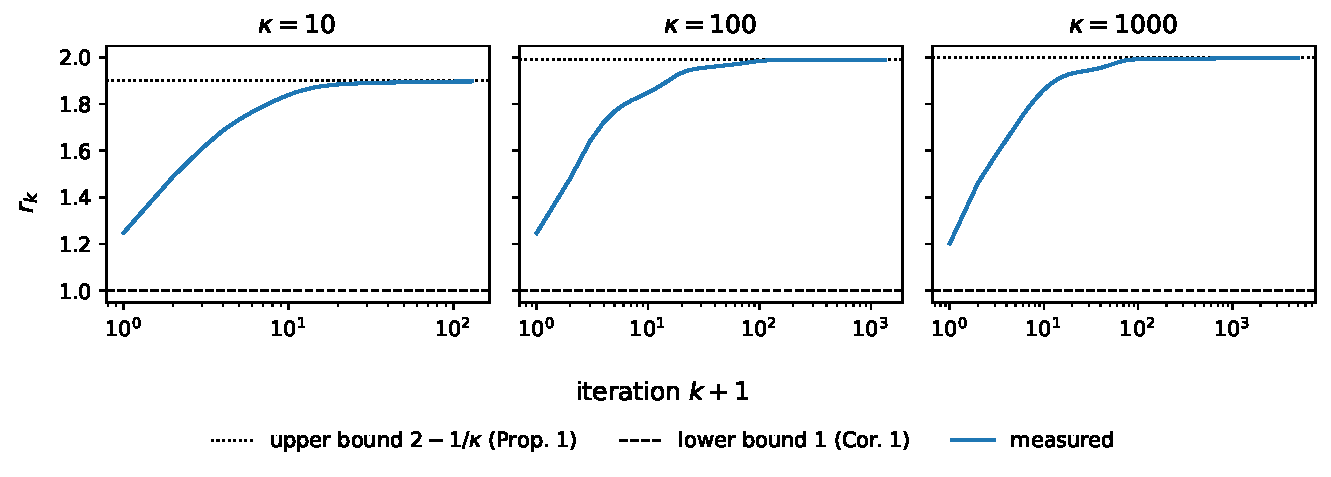
\includegraphics[width=\textwidth]{../code/figures/fig01a_rk.pdf}
\caption{Ratio $r_k$ between the actual decrease $f(x_k) - f(x_{k+1})$ and the decrease $\frac{1}{2L}\norm{\nabla f(x_k)}^2$ guaranteed by Corollary~\ref{cor:sufficient}, for $\kappa \in \{10, 100, 1000\}$ (logarithmic horizontal axis). Dashed line: lower bound $1$ (Corollary~\ref{cor:sufficient}). Dotted line: upper bound $2 - 1/\kappa$ (Proposition~\ref{prop:rk}).}
\label{fig:rk}
\end{figure}

\paragraph{Tightness of the sufficient decrease (Figure~\ref{fig:rk}).}
For the three values of $\kappa$, the ratio $r_k$ stays in the interval $[1, 2 - 1/\kappa]$ predicted by Proposition~\ref{prop:rk}. It starts at $r_0 \approx 1.25$ for $\kappa = 10$ and $\kappa = 100$, and $r_0 \approx 1.20$ for $\kappa = 1000$: at the first iterations, the guaranteed decrease of Corollary~\ref{cor:sufficient} is close to the actual one. Then $r_k$ increases towards its upper bound: the maximal observed values are $1.8971$, $1.9900$ and $1.9990$, for upper bounds $1.9$, $1.99$ and $1.999$. For $\kappa = 10$, the remaining gap of order $3 \times 10^{-3}$ is due to the eigenvalue $\lambda_2 \approx 1.03$, very close to $\mu$, whose component has not yet vanished when the run is stopped by the threshold $10^{-12}$ (after $130$ iterations). This is the behaviour anticipated in the remark following Proposition~\ref{prop:rk}: the components of $x_k$ along eigenvectors with large eigenvalues are damped quickly, so that $g_k = A x_k$ aligns with the eigenvectors of the smallest eigenvalues, and the Rayleigh quotient $\ip{g_k}{Ag_k}/\norm{g_k}^2$ decreases towards $\mu$. For $\kappa = 1000$, the convergence to $2 - 1/\kappa$ goes through an intermediate regime: the next smallest eigenvalue is $\lambda_2 \approx 6.73$, and the component along its eigenvector only decays by a factor $(1 - \lambda_2/L)/(1 - \mu/L)$ per step relative to the slowest one, that is about $0.57\%$. Accordingly, $r_k \approx 1.992$ at $k = 100$, close to $2 - \lambda_2/L \approx 1.993$, and $r_k$ only reaches $1.9988$ around $k = 1000$. 

\begin{figure}[ht]
\centering
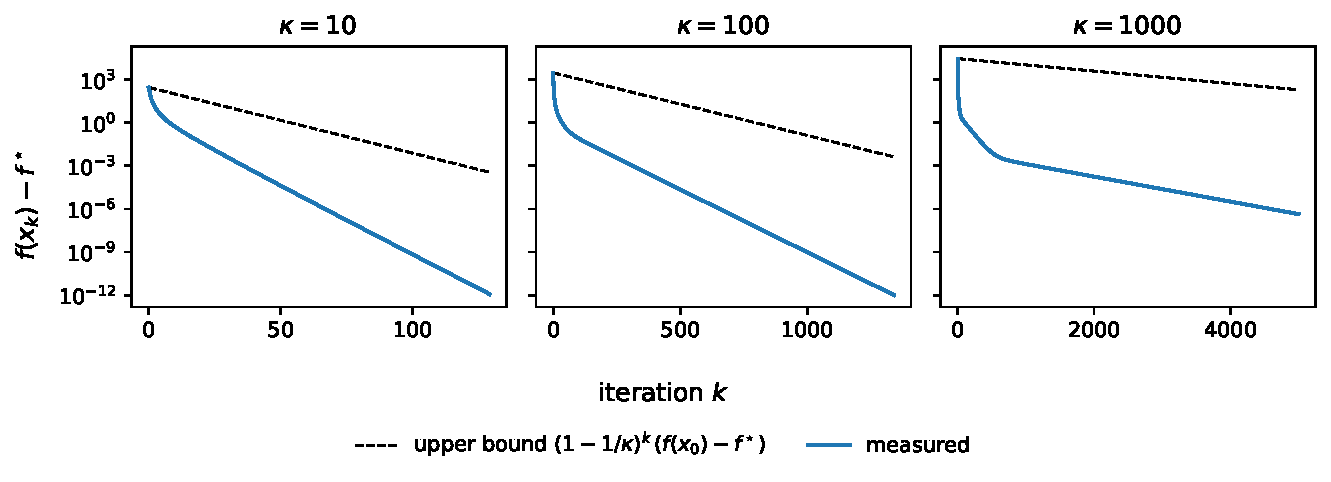
\includegraphics[width=\textwidth]{../code/figures/fig01b_gap.pdf}
\caption{Optimality gap $f(x_k) - f^\star$ of gradient descent with step size $1/L$ (logarithmic vertical axis), for $\kappa \in \{10, 100, 1000\}$. Dashed line: upper bound $(1 - 1/\kappa)^k \big(f(x_0) - f^\star\big)$.}
\label{fig:gap}
\end{figure}

\paragraph{Convergence rate (Figure~\ref{fig:gap}).}
The measured gap always stays below the bound $(1 - 1/\kappa)^k (f(x_0) - f^\star)$. After a short initial phase, in which the components along large eigenvalues vanish, each curve is a straight line in logarithmic scale: the convergence is linear, and its rate deteriorates as $\kappa$ grows. However, the measured slope is about twice the slope of the bound. Table~\ref{tab:slopes} compares the slope of $\log f(x_k)$, fitted by least squares on the second half of the plotted iterations, with the slope $\log(1 - 1/\kappa)$ of the bound. For instance, for $\kappa = 10$, the gap reaches about $10^{-12}$ after $130$ iterations, while the bound is still of order $4 \times 10^{-4}$.

\begin{table}[ht]
\centering
\begin{tabular}{cccc}
\hline
$\kappa$ & measured slope & $\log(1 - 1/\kappa)$ & ratio \\
\hline
$10$ & $-0.2186$ & $-0.1054$ & $2.07$ \\
$100$ & $-0.0201$ & $-0.0101$ & $2.00$ \\
$1000$ & $-0.0020$ & $-0.0010$ & $2.00$ \\
\hline
\end{tabular}
\caption{Slope of $\log\big(f(x_k) - f^\star\big)$ as a function of $k$, compared with the slope of the theoretical bound.}
\label{tab:slopes}
\end{table}

This factor $2$ has a simple heuristic explanation. Writing $x_k = \sum_i c_i^{(k)} e_i$ in an orthonormal eigenbasis of $A$, each component satisfies $c_i^{(k)} = (1 - \lambda_i/L)^k c_i^{(0)}$, so that
\[
f(x_k) = \frac12 \sum_{i=1}^d \lambda_i \Big(1 - \frac{\lambda_i}{L}\Big)^{2k} \big(c_i^{(0)}\big)^2 ,
\]
which, for large $k$, behaves like $C\,(1 - 1/\kappa)^{2k}$ as soon as $c_1^{(0)} \neq 0$. The exponent $2k$ comes from the fact that $f$ is quadratic in $x$; the general bound, which only uses smoothness and strong convexity, loses this square. A rigorous statement is left for a forthcoming proposition.

\paragraph{Conclusion.}
On quadratics, the theory correctly predicts the qualitative behaviour of gradient descent: the sufficient decrease holds at every step, the convergence is linear and slows down as $\kappa$ grows. Quantitatively, Proposition~\ref{prop:rk} describes the ratio $r_k$ exactly, whereas the general bound on $f(x_k) - f^\star$ is pessimistic by a factor $2$ in the exponent. Whether this pessimism persists in the worst case over all $L$-smooth and $\mu$-strongly convex functions is a natural question, which can be investigated with performance estimation techniques.

\emph{[Further experiments: logistic regression; non-convex PL example; SGD on least squares; comparison with Adam.]}

\section{Discussion}
\emph{[Where the bounds are tight, where they are pessimistic, and why.]}

\begin{thebibliography}{9}
\bibitem{garrigos} G.~Garrigos and R.~M.~Gower. \emph{Handbook of Convergence Theorems for (Stochastic) Gradient Methods}. arXiv:2301.11235, 2023.
\bibitem{bubeck} S.~Bubeck. \emph{Convex Optimization: Algorithms and Complexity}. Foundations and Trends in Machine Learning, 2015.
\bibitem{nesterov} Y.~Nesterov. \emph{Lectures on Convex Optimization}. Springer, 2nd edition, 2018.
\bibitem{karimi} H.~Karimi, J.~Nutini and M.~Schmidt. Linear convergence of gradient and proximal-gradient methods under the Polyak--{\L}ojasiewicz condition. \emph{ECML PKDD}, 2016.
\bibitem{su} W.~Su, S.~Boyd and E.~J.~Cand\`es. A differential equation for modeling Nesterov's accelerated gradient method. \emph{NeurIPS}, 2014.
\end{thebibliography}

\end{document}
